\chapter{Конструкторская часть}

В этом разделе будут представлены требования к программному обес-
печению (ПО) и схема алгоритмов.

\section{Требования к программному обеспечению}

К программе предъявлен ряд требований:

\begin{enumerate}
	\item наличие интерфейса для выбора действий;
	\item возможность выбора алгоритма решения задачи коммивояжера. 
\end{enumerate}

\section{Разработка алгоритма полного перебора}

На рисунке~\ref{fig:brute_force} представлен алгоритм полного перебора.

\begin{figure}[h!]
	\centering{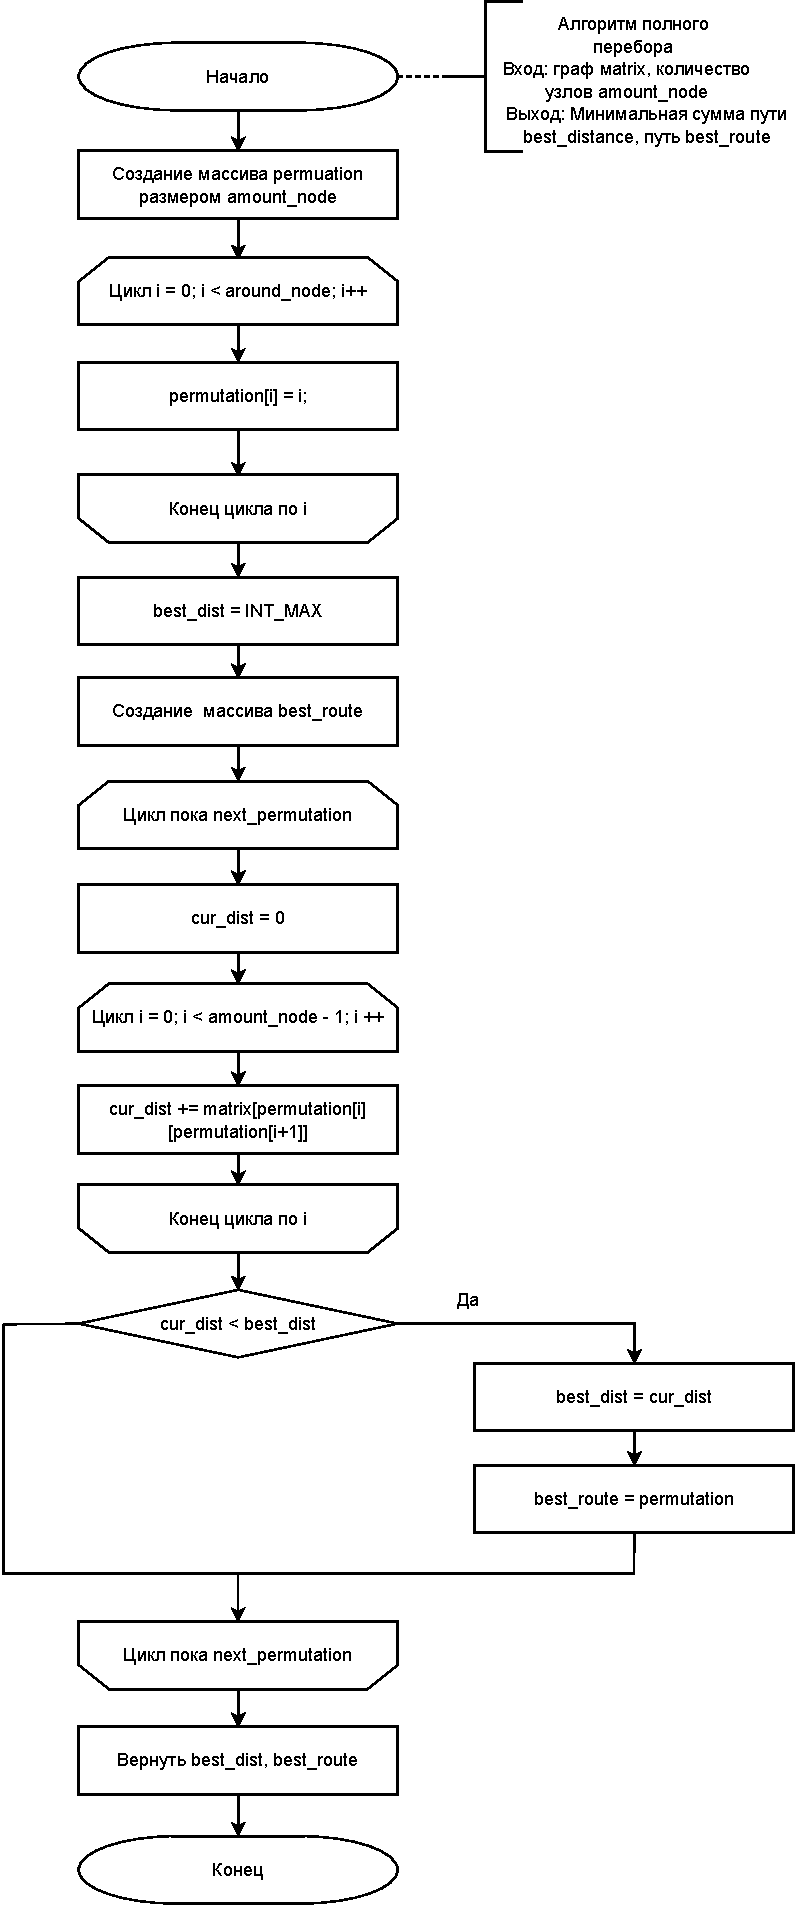
\includegraphics[scale=0.7]{photos/brute_force.pdf}}
	\caption{Алгоритм полного перебора}
	\label{fig:brute_force}
\end{figure}

\clearpage

\section{Разработка муравьиного алгоритма}

На рисунке~\ref{fig:calcQ} представлен алгоритм вычисления среднего значения расстояний между всеми парами.

\begin{figure}[h!]
	\centering{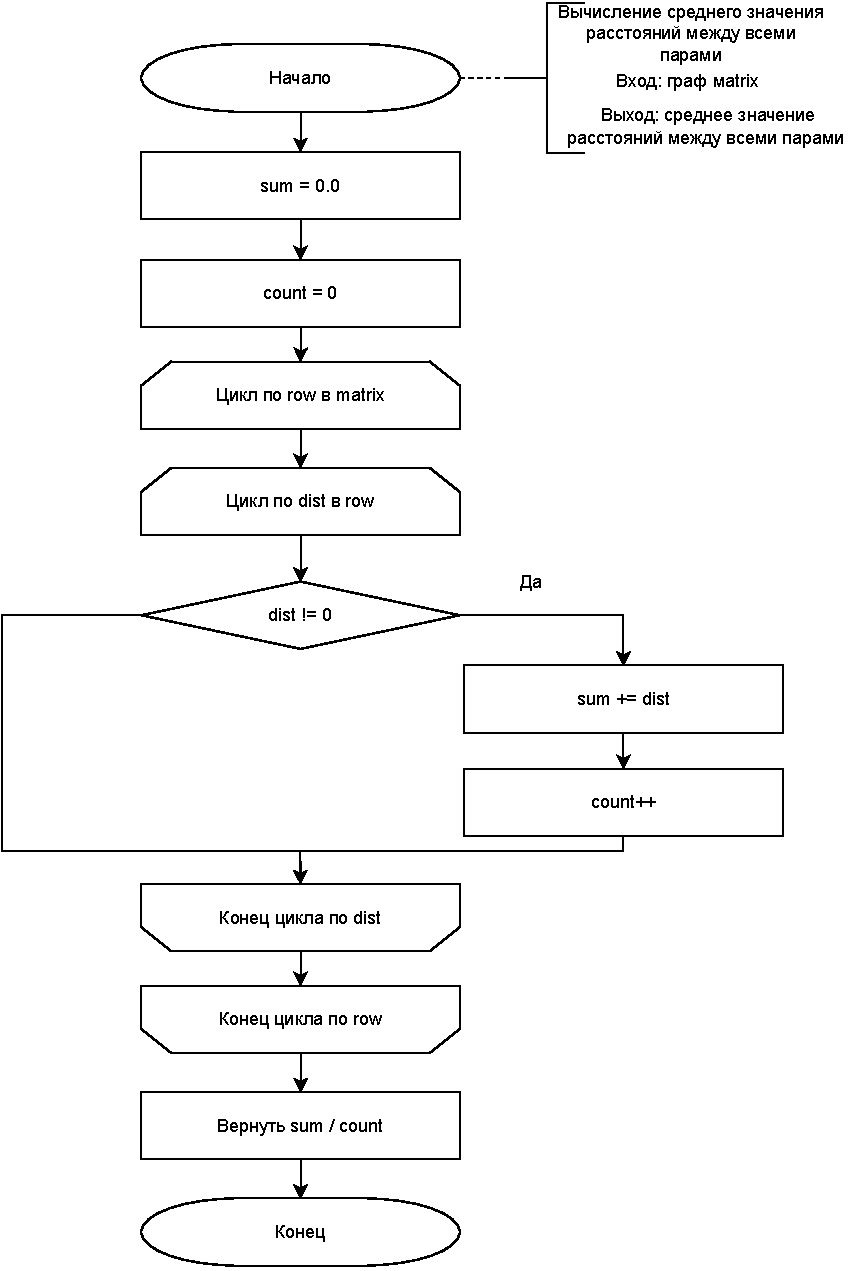
\includegraphics[scale=0.9]{photos/calcQ.pdf}}
	\caption{Алгоритм вычисления среднего значения расстояний между всеми парами}
	\label{fig:calcQ}
\end{figure}

\clearpage

На рисунке~\ref{fig:chooseNextLoc} представлен алгоритм выбора следующего города, куда муравей должен переместиться.

\begin{figure}[h!]
	\centering{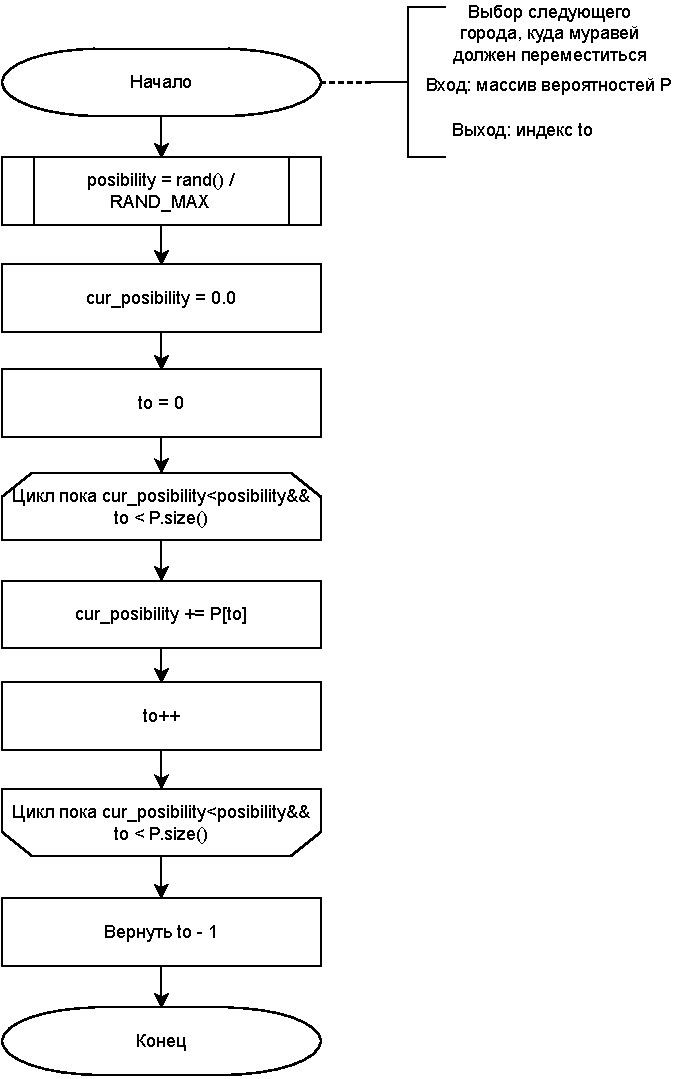
\includegraphics[scale=0.9]{photos/chooseNextLoc.pdf}}
	\caption{Алгоритм выбора следующего города, куда муравей должен переместиться}
	\label{fig:chooseNextLoc}
\end{figure}

\clearpage

На рисунке~\ref{fig:calcLen} представлен алгоритм вычисления пути, пройденного муравьем.

\begin{figure}[h!]
	\centering{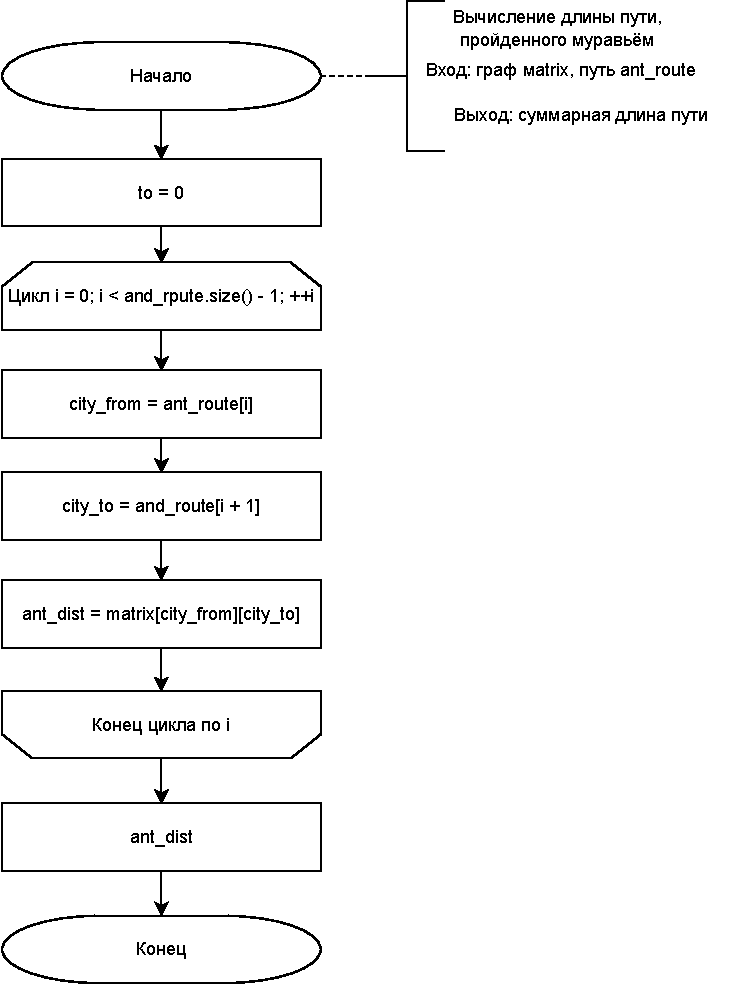
\includegraphics[scale=0.9]{photos/calcLen.pdf}}
	\caption{Алгоритм вычисления пути, пройденного муравьем}
	\label{fig:calcLen}
\end{figure}

На рисунке~\ref{fig:ant} представлен муравьиный алгоритм.

\begin{figure}[h!]
	\centering{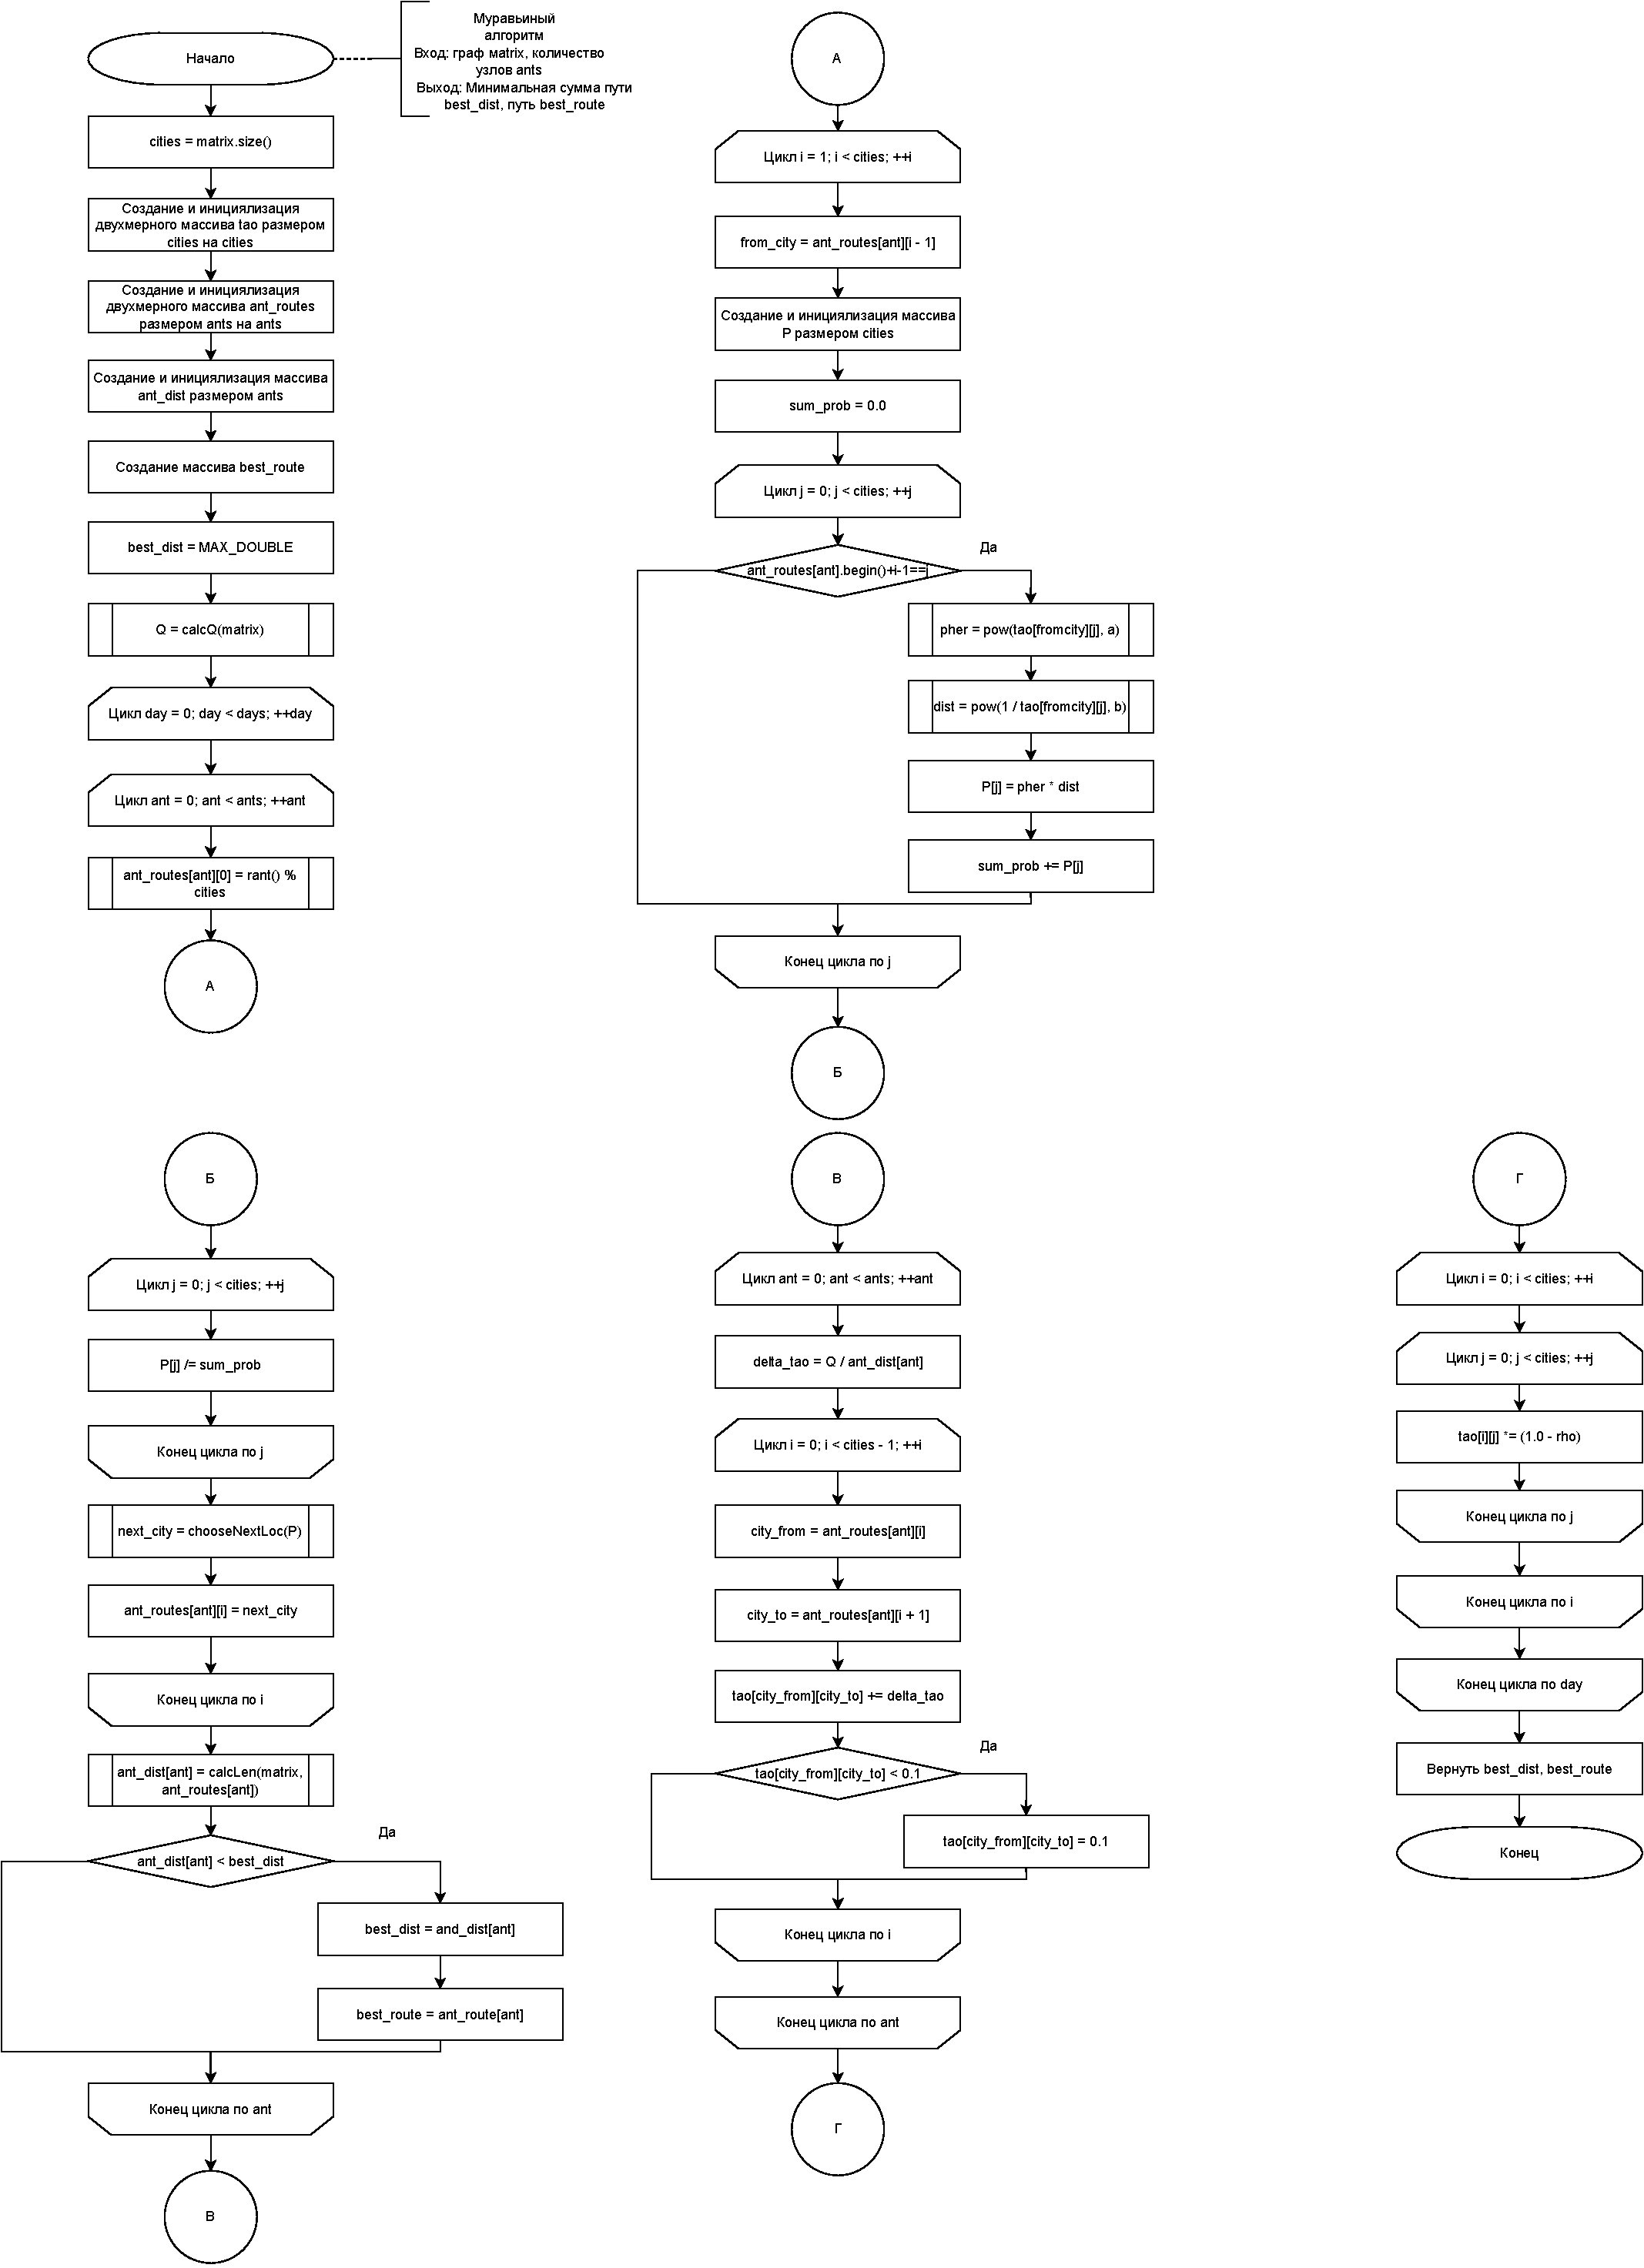
\includegraphics[scale=0.5]{photos/ant.pdf}}
	\caption{Муравьиный алгоритм}
	\label{fig:ant}
\end{figure}

\clearpage

\section*{Вывод}

В данном разделе были перечислены требования к программному обеспечению и построены схемы алгоритмов решения задачи коммивояжера.
